\chapter{Representing IACT data}
%
IACTs aim at reconstructing the energy, source position and particle type of
cosmic rays via their Cherenkov-light. The Cherenkov-light flashes that are
only nano seconds in duration are measured and can be separated from background
light from stars or ambient light by their brightness and topology within the
camera image. There are different ways to represent air shower data. FACT uses
the so called main-pulse representation, whereas this work focuses on a novel
data format, both of which are described in the following chapter.

\section{The Main-Pulse representation}
%
Data taken by an Imaging-Air-Cherenkov-Telescope
(IACT), like FACT, is usually represented in so called time series.
These time series owe their name to the fact that they represent voltages at the photosensors over time. Within these time series lie so called main-pulses that represent the increased voltage that a charge deposition of an air-shower causes. So by looking for those main-pulses shower events can be found upon the detector noise and ambient light in the camera. Of course, the main-pulses consist of multiple photon signals and noise superposed over time, but in this state they are electric pulses representing the response of very specific hardware. So rather than measuring physical properties, this means that the charge deposit has to be interpretated to be transferred into physics observables, independant of these specifics \textbf{[which ones?]}. Such interpretations always include assumptions of physical and technical kinds. By integrating the charge in one pixel an equivalent of a photon count can be obtained, called the \textit{photon equivalent} (PE). So the first observable in this representation is the PE which corresponds to the best estimate of the number of photons measured per pixel. The photon counts are spatially located by the corresponding pixel they are assigned to. The 1440 pixels of FACT are the determining grid that yield the spatial coordinates of every shower event.

The second observable is the time. When the telescope is triggered and records
data the arrival time of the event is measured via the time information within
the time series. From the time series a quantized timing information per pixel
can be developed by dividing the event into time slices. From this the arrival
time of the photons per pixel can be calculated by averaging. Thus, the arrival
times $t$ per pixel are the second observable of the main-pulse event
representation, besides the photon-equivalents.

\begin{figure}
  \begin{subfigure}{0.475\textwidth}
    \includegraphics[width=1.1\textwidth, page=40]{Plots/cleaning_facttools_pe_20131104_162.pdf}
  \end{subfigure}
  \begin{subfigure}{0.475\textwidth}
    \includegraphics[width=1.1\textwidth, page=40]{Plots/cleaning_facttools_arrival_times_20131104_162.pdf}
  \end{subfigure}
  \caption{The measured observables of the main-pulse representation are shown as scatter plots within the pixels. On the left the distribution of photon-equivalents $c$ of a typical shower event (Crab observation on November, 4th 2013, run 162, event 80) is shown. On the right the arrival times of that event's photons with respect to the mean arrival time in ns are displayed.}
  \label{fig:mainpulse}
\end{figure}

\section{The PhotonStream representation}

The Photonstream representation aims at creating a data format consisting of photons by storing their observed physical properties. So from the measured time series single photons are extracted instead of deriving photon counts in pixels. Each of these photons is assigned an arrival time and pixel, creating a list of arrival times per photon for each pixel. By doing so, a 3-dimensional data set is created, which can be represented in form of so called point clouds (\autoref{fig:event}).
%
\begin{figure}
  \centering
  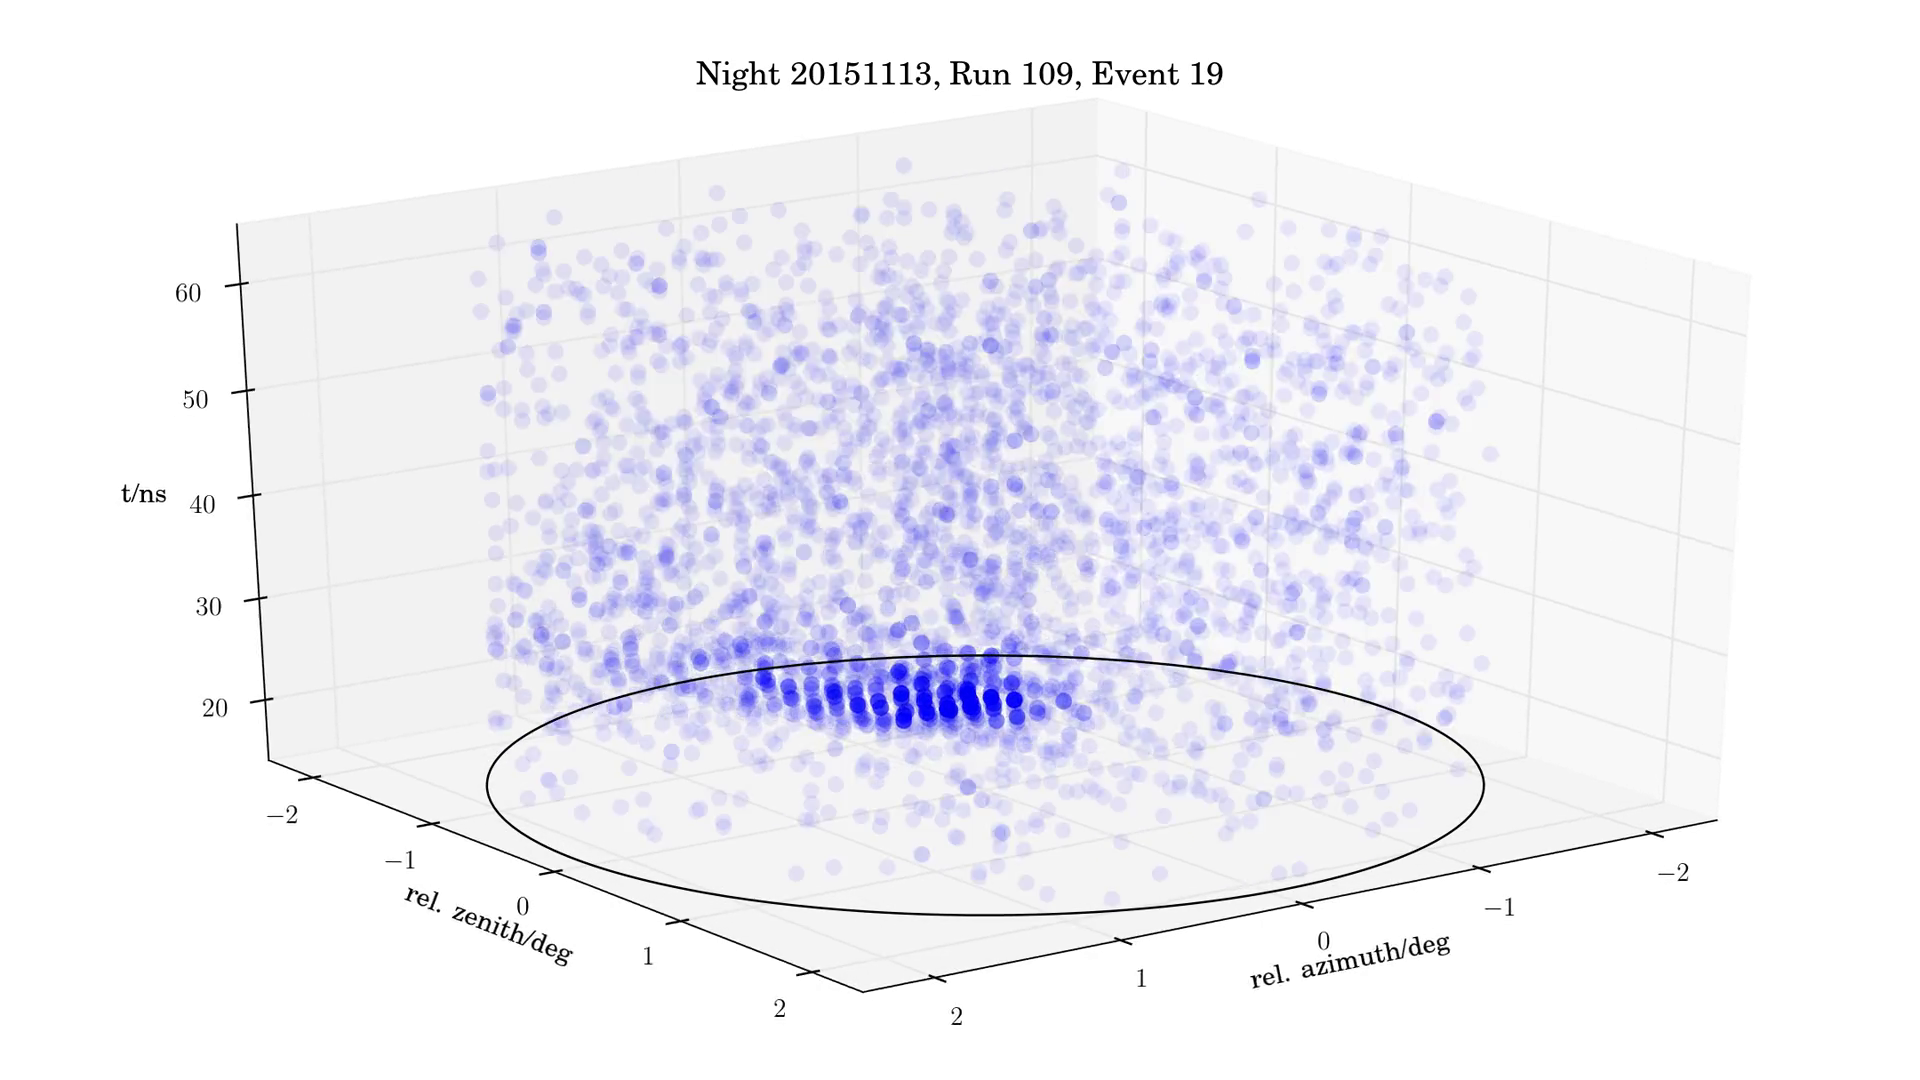
\includegraphics[width=1.1\textwidth]{Plots/event2.png}
  \caption{Uncleaned event represented by the 3-dimensional point cloud of the Photonstream. Every blue sphere represents a measured photon in the corresponding time slice and pixel.}
  \label{fig:event}
\end{figure}
